\section{Desarrolo}

\subsection{Discretización}
El problema de Navier Stokes es gobernado por la siguiente escuación

$$\frac{\partial \vec{v}}{\partial t}+(\vec{v}\cdot\nabla)\vec{v}=-\frac{1}{\rho}\nabla p + \nu \nabla^2\vec{v}$$


Los operadores presentes en la primera ecuación presentada, al ser usados en su forma bidimencional, permiten una reescritura como la siguiente:

$$\frac{\partial u}{\partial t}+u\frac{\partial u}{\partial x}+v\frac{\partial u}{\partial y} = -\frac{1}{\rho}\frac{\partial p}{\partial x}+\nu \left(\frac{\partial^2 u}{\partial x^2}+\frac{\partial^2 u}{\partial y^2} \right)$$

$$\frac{\partial v}{\partial t}+u\frac{\partial v}{\partial x}+v\frac{\partial v}{\partial y} = -\frac{1}{\rho}\frac{\partial p}{\partial y}+\nu\left(\frac{\partial^2 v}{\partial x^2}+\frac{\partial^2 v}{\partial y^2}\right)$$

$$\frac{\partial^2 p}{\partial x^2}+\frac{\partial^2 p}{\partial y^2} = -\rho\left(\frac{\partial u}{\partial x}\frac{\partial u}{\partial x}+2\frac{\partial u}{\partial y}\frac{\partial v}{\partial x}+\frac{\partial v}{\partial y}\frac{\partial v}{\partial y} \right)$$

Las primeras dos ecuaciones se corresponden con la velocidad en las direcciones en x e y, mientras que la tercera da cuenta de los efectos de la presión.

Comenzaremos con algunas definiciones. Al modelar con diferencias finitas, se utilizan ciertos reemplazos de los operadores diferenciales conocidos como discretizaciones. Como su nombre indica, estas son versiones discretas de los operadores, y se las usa bajo el supuesto de que en el límite se comportan de forma similar. Pasaremos ahora a definir algunas discretizaciones que serán utilizadas para modelar el problema.
~\\
~\\
\begin{minipage}{\linewidth}

Centradas de primer orden:
\begin{center}

~\\
$\frac{dU}{dx} = \frac{U^{n}_{i+1,j} - U^{n}_{i-1,j}}{2dx} $
~\\
~\\
$\frac{dU}{dy} = \frac{U^{n}_{i,j+1} - U^{n}_{i,j-1}}{2dy} $
~\\
~\\
$\frac{dU}{dt} = \frac{U^{n+1}_{i,j} - U^{n-1}_{i,j}}{2dt} $
~\\
\end{center}

\end{minipage}
\begin{minipage}{\linewidth}



Centradas de segundo orden:
\begin{center}

~\\
$\frac{d^{2}U}{dx^{2}} = \frac{ U^{n}_{i+1,j} - 2*U^{n}_{i,j} + U^{n}_{i-1,j}}{dx^2}$
~\\
~\\
$\frac{d^{2}U}{dy^{2}} = \frac{ U^{n}_{i,j+1} - 2*U^{n}_{i,j} + U^{n}_{i,j-1}}{dx^2}$
~\\
~\\
$\frac{d^{2}U}{dt^{2}} = \frac{ U^{n+1}_{i,j} - 2*U^{n}_{i,j} + U^{n-1}_{i,j}}{dt^2}$
~\\
\end{center}

\end{minipage}
\begin{minipage}{\linewidth}

Adelantadas de primer orden:
\begin{center}

~\\
$\frac{dU}{dx} = \frac{U^{n}_{i+1,j} - U^{n}_{i,j}}{dx} $
~\\
~\\
$\frac{dU}{dy} = \frac{U^{n}_{i,j+1} - U^{n}_{i,j}}{dy} $
~\\
~\\
$\frac{dU}{dt} = \frac{U^{n+1}_{i,j} - U^{n}_{i,j}}{dx} $
~\\
\end{center}

\end{minipage}
\begin{minipage}{\linewidth}


Atrasadas de primer orden:
\begin{center}

~\\
$\frac{dU}{dx} = \frac{U^{n}_{i,j} - U^{n}_{i-1,j}}{dx} $
~\\
~\\
$\frac{dU}{dy} = \frac{U^{n}_{i,j} - U^{n}_{i,j-1}}{dy} $
~\\
~\\
$\frac{dU}{dt} = \frac{U^{n}_{i,j} - U^{n-1}_{i,j}}{dx} $
~\\
\end{center}
\end{minipage}
~\\

\begin{minipage}{\linewidth}

Reemplazando estas discretizaciones en las ecuaciones semi-acopladas de Navier Stokes obtenemos: 
\begin{center}
~\\

~\\
$\frac{u_{i,j}^{n+1}-u_{i,j}^{n}}{\Delta t}+u_{i,j}^{n}\frac{u_{i,j}^{n}-u_{i-1,j}^{n}}{\Delta x}+v_{i,j}^{n}\frac{u_{i,j}^{n}-u_{i,j-1}^{n}}{\Delta y}
=-\frac{1}{\rho}\frac{p_{i+1,j}^{n}-p_{i-1,j}^{n}}{2\Delta x}+\nu (\frac{u_{i+1,j}^{n}-2u_{i,j}^{n}+u_{i-1,j}^{n}}{\Delta x^2}+\frac{u_{i,j+1}^{n}-2u_{i,j}^{n}+u_{i,j-1}^{n}}{\Delta y^2}) + Fu$
~\\
~\\
~\\

$\frac{v_{i,j}^{n+1}-v_{i,j}^{n}}{\Delta t}+u_{i,j}^{n}\frac{v_{i,j}^{n}-v_{i-1,j}^{n}}{\Delta x}+v_{i,j}^{n}\frac{v_{i,j}^{n}-v_{i,j-1}^{n}}{\Delta y}=-\frac{1}{\rho}\frac{p_{i,j+1}^{n}-p_{i,j-1}^{n}}{2\Delta y}
+\nu(\frac{v_{i+1,j}^{n}-2v_{i,j}^{n}+v_{i-1,j}^{n}}{\Delta x^2}+\frac{v_{i,j+1}^{n}-2v_{i,j}^{n}+v_{i,j-1}^{n}}{\Delta y^2}) + Fv$
~\\
~\\
~\\

$\frac{p_{i+1,j}^{n}-2p_{i,j}^{n}+p_{i-1,j}^{n}}{\Delta x^2}+\frac{p_{i,j+1}^{n}-2*p_{i,j}^{n}+p_{i,j-1}^{n}}{\Delta y^2} 
=\rho[\frac{1}{\Delta t}(\frac{u_{i+1,j}-u_{i-1,j}}{2\Delta x}+\frac{v_{i,j+1}-v_{i,j-1}}{2\Delta y})$
\end{center}

\end{minipage}
~\\
~\\

\begin{minipage}{\linewidth}
Aquí en la última ecuación podemos ver que no se reemplazó directamente cada operador mediante las ecuaciones de discretización, sino que se agregó un término temporal, sin que hubiera en principio información sobre el tiempo en la ecuación de la presión. Este cambio se hace con el objetivo de acoplar la ecuación de la presión con las ecuaciones de velocidad. El mecanismo por el cual la adición de este nuevo término acopla las ecuaciones, no se presentará en este trabajo.
~\\

Cabe aclarar que al discretizar, se puede modelar el sistema mediante un método implícito o explícito. Un método implícito, o parcialmente implícito, incluiría una ponderación entre los valores de las variables en la iteración n, y la iteración n+1. En este trabajo utilizaremos un método explícito, ya que el sistema de ecuaciones determinado por un método explícito es lineal, y resulta en relaciones donde un elemento en la iteración n+1 depende de otros en la iteración n, pudiendo entonces realizarse los reemplazos en las matrices que representan el sistema de forma directa, y resultando así en una implementación con menor dependencia de datos. Un método implícito da como resultado un sistema no lineal, en el cual hay que hacer uso de algún método de resolución de sistemas no lineales, como punto fijo, lo cual aumenta la complejidad de la implementación.

\end{minipage}

\newpage

\subsection{Implementación}
La implementación fue realizada completamente en C++, excepto por la sección donde es crítico el rendimiento, la cual fue programada en C++ y Assembler. Esta sección es la correspondiente a la función \textit{calcVelocities}, que como su nombre indica, calcula las velocidades en cada punto.
~\\
~\\
El programa define las matrices U1, U2, V1, V2, P1, P2, que representan el estado del sistema en una iteración para la velocidad en \textit{u}, en \textit{v}, y la presión, y luego estas mismas en la iteración siguiente. 
~\\
~\\
Se definen las condiciones iniciales del problema, y luego se utiliza un método explícito para calcular los nuevos valores del sistema. Estos son guardados en U2, V2, y P2. Seguido de esto, el programa reemplaza los valores de U1, V1, y P1, por aquellos de U2, V2 y P2, quedado así preparado para la siguiente iteración. 
~\\
~\\
Se implementó también una clase mat2, que representa una matriz, y que contiene un puntero a un arreglo de números de punto flotante de precisión simple y dos enteros que representan el tamaño en filas y columnas de la matriz. Además la clase cuenta con funciones que realizan la abstracción de indexar en el arreglo calculando la posición del elemento buscado como la columna pedida, más la fila pedida multiplicada por la cantidad de columnas. 
~\\
~\\
En cuanto a la vectorización, como se comentó anteriormente se utilizó la tecnología SIMD de Intel, de la forma descripta a continuación:
\begin{itemize}
	\item Mediante una directiva DEFINE presente en el Makefile, se elije si se desea compilar con soporte para SIMD, soporte para OpenMP, ambos, o ninguno.

	\item El programa define las matrices necesarias con los valores iniciales según lo estipulado por el método de discretización utilizado.

	\item La sección del programa que realiza el cálculo consta de tres ciclos consecutivos. El primero cicla en la variable \textit{t}, que representa el tiempo, el segundo en la variable \textit{i}, que representa la altura, y el tercero en la variable \textit{j} que representa el ancho.
	
    \item La paralelización mediante OpenMP se realiza en la variable \textit{i}.
	
    \item La vectorización mediante SIMD, se realiza en la variable \textit{j}. Es decir, en un solo llamado a la versión de Assembler de la función de cálculo se procesan 4 elementos consecutivos en memoria.

    \item Además, al utilizar SIMD, cuando se llega a un valor de \textit{j} menor al ancho de los registros XMM dividido por el tamaño del tipo de datos flotante de presición simple, se cambia el procesamiento mediante SIMD por el de C++, hasta que \textit{j} alcanza su valor máximo.

	\item Además, durante la simulación no se crean ni se destruyen matrices, sino que estas son reutilizadas cambiando los valores que contienen para no perder tiempo manejando memoria.
\end{itemize}

Los resultados de la simulación pueden apreciarse en las \textbf{Figuras \ref{fig:run_1}} y la \textbf{Figuras \ref{fig:run_2}}

~\\
\begin{figure}[!htbp]
\centering
\begin{subfigure}{.3\textwidth}
  \centering
  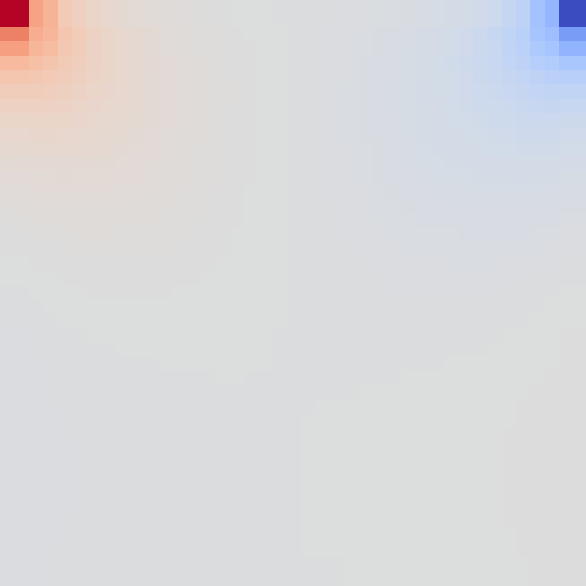
\includegraphics[width=.8\linewidth]{imagenes/small_p.png}
  \caption{Presion}
  \label{fig:sub1}
\end{subfigure}%
\begin{subfigure}{.3\textwidth}
  \centering
  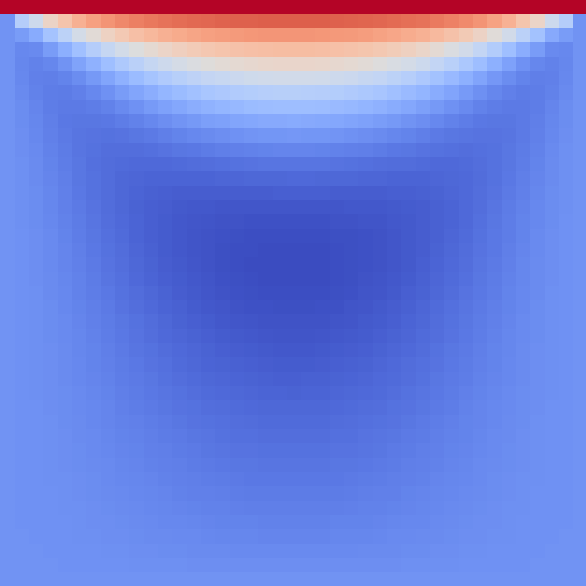
\includegraphics[width=.8\linewidth]{imagenes/small_u.png}
  \caption{Velocidad en x}
  \label{fig:sub2}
\end{subfigure}
\begin{subfigure}{.3\textwidth}
  \centering
  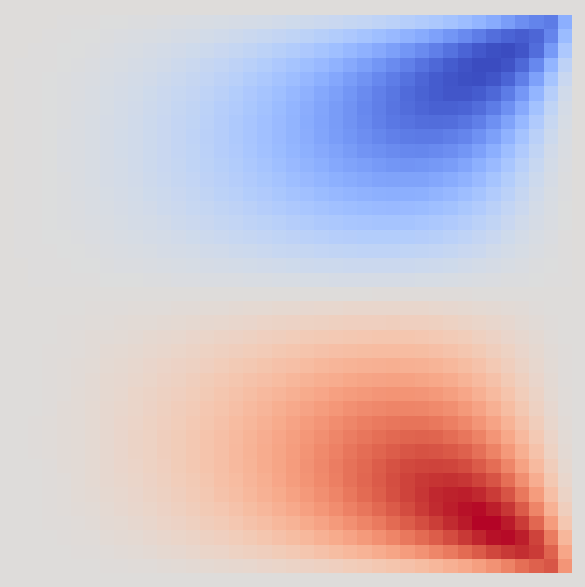
\includegraphics[width=.8\linewidth]{imagenes/small_v.png}
  \caption{Velocidad en y}
  \label{fig:sub2}
\end{subfigure}
\caption{Velocidad y presión}
\label{fig:run_1}
\end{figure}
\begin{figure}[!htbp]
\centering
\begin{subfigure}{.3\textwidth}
  \centering
  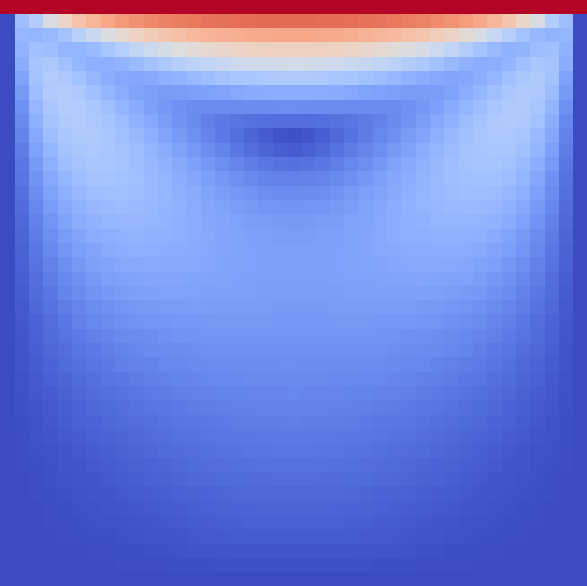
\includegraphics[width=.8\linewidth]{imagenes/small_norm.png}
  \caption{Norma de la velocidad}
  \label{fig:sub1}
\end{subfigure}%
\begin{subfigure}{.3\textwidth}
  \centering
  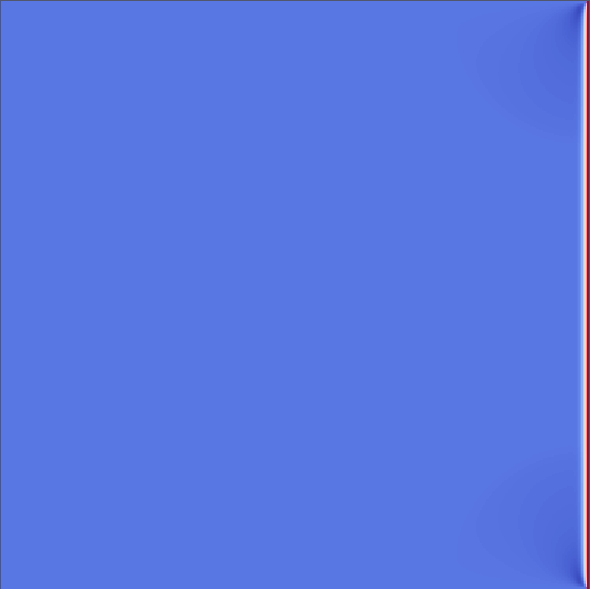
\includegraphics[width=.8\linewidth]{imagenes/u.png}
  \caption{Velocidad en x}
  \label{fig:sub2}
\end{subfigure}
\begin{subfigure}{.3\textwidth}
  \centering
  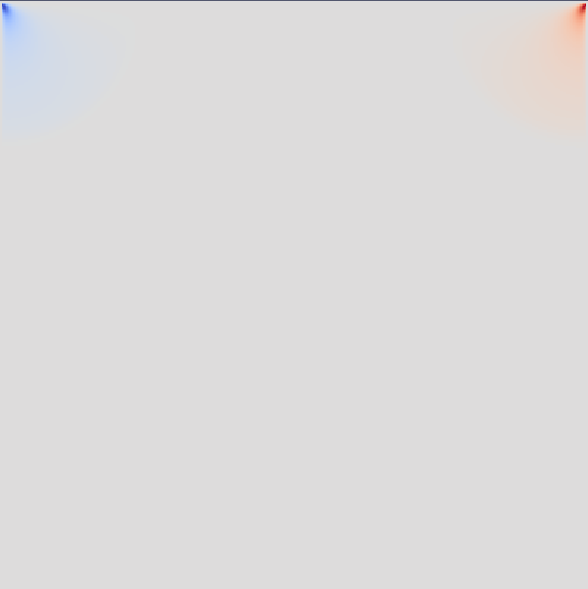
\includegraphics[width=.8\linewidth]{imagenes/v.png}
  \caption{Velocidad en y}
  \label{fig:sub2}
\end{subfigure}
\caption{Norma y velocidades con mayor resolución}
\label{fig:run_2}
\end{figure}
